\documentclass[1p]{elsarticle_modified}
%\bibliographystyle{elsarticle-num}

%\usepackage[colorlinks]{hyperref}
%\usepackage{abbrmath_seonhwa} %\Abb, \Ascr, \Acal ,\Abf, \Afrak
\usepackage{amsfonts}
\usepackage{amssymb}
\usepackage{amsmath}
\usepackage{amsthm}
\usepackage{scalefnt}
\usepackage{amsbsy}
\usepackage{kotex}
\usepackage{caption}
\usepackage{subfig}
\usepackage{color}
\usepackage{graphicx}
\usepackage{xcolor} %% white, black, red, green, blue, cyan, magenta, yellow
\usepackage{float}
\usepackage{setspace}
\usepackage{hyperref}

\usepackage{tikz}
\usetikzlibrary{arrows}

\usepackage{multirow}
\usepackage{array} % fixed length table
\usepackage{hhline}

%%%%%%%%%%%%%%%%%%%%%
\makeatletter
\renewcommand*\env@matrix[1][\arraystretch]{%
	\edef\arraystretch{#1}%
	\hskip -\arraycolsep
	\let\@ifnextchar\new@ifnextchar
	\array{*\c@MaxMatrixCols c}}
\makeatother %https://tex.stackexchange.com/questions/14071/how-can-i-increase-the-line-spacing-in-a-matrix
%%%%%%%%%%%%%%%

\usepackage[normalem]{ulem}

\newcommand{\msout}[1]{\ifmmode\text{\sout{\ensuremath{#1}}}\else\sout{#1}\fi}
%SOURCE: \msout is \stkout macro in https://tex.stackexchange.com/questions/20609/strikeout-in-math-mode

\newcommand{\cancel}[1]{
	\ifmmode
	{\color{red}\msout{#1}}
	\else
	{\color{red}\sout{#1}}
	\fi
}

\newcommand{\add}[1]{
	{\color{blue}\uwave{#1}}
}

\newcommand{\replace}[2]{
	\ifmmode
	{\color{red}\msout{#1}}{\color{blue}\uwave{#2}}
	\else
	{\color{red}\sout{#1}}{\color{blue}\uwave{#2}}
	\fi
}

\newcommand{\Sol}{\mathcal{S}} %segment
\newcommand{\D}{D} %diagram
\newcommand{\A}{\mathcal{A}} %arc


%%%%%%%%%%%%%%%%%%%%%%%%%%%%%5 test

\def\sl{\operatorname{\textup{SL}}(2,\Cbb)}
\def\psl{\operatorname{\textup{PSL}}(2,\Cbb)}
\def\quan{\mkern 1mu \triangleright \mkern 1mu}

\theoremstyle{definition}
\newtheorem{thm}{Theorem}[section]
\newtheorem{prop}[thm]{Proposition}
\newtheorem{lem}[thm]{Lemma}
\newtheorem{ques}[thm]{Question}
\newtheorem{cor}[thm]{Corollary}
\newtheorem{defn}[thm]{Definition}
\newtheorem{exam}[thm]{Example}
\newtheorem{rmk}[thm]{Remark}
\newtheorem{alg}[thm]{Algorithm}

\newcommand{\I}{\sqrt{-1}}
\begin{document}

%\begin{frontmatter}
%
%\title{Boundary parabolic representations of knots up to 8 crossings}
%
%%% Group authors per affiliation:
%\author{Yunhi Cho} 
%\address{Department of Mathematics, University of Seoul, Seoul, Korea}
%\ead{yhcho@uos.ac.kr}
%
%
%\author{Seonhwa Kim} %\fnref{s_kim}}
%\address{Center for Geometry and Physics, Institute for Basic Science, Pohang, 37673, Korea}
%\ead{ryeona17@ibs.re.kr}
%
%\author{Hyuk Kim}
%\address{Department of Mathematical Sciences, Seoul National University, Seoul 08826, Korea}
%\ead{hyukkim@snu.ac.kr}
%
%\author{Seokbeom Yoon}
%\address{Department of Mathematical Sciences, Seoul National University, Seoul, 08826,  Korea}
%\ead{sbyoon15@snu.ac.kr}
%
%\begin{abstract}
%We find all boundary parabolic representation of knots up to 8 crossings.
%
%\end{abstract}
%\begin{keyword}
%    \MSC[2010] 57M25 
%\end{keyword}
%
%\end{frontmatter}

%\linenumbers
%\tableofcontents
%
\newcommand\colored[1]{\textcolor{white}{\rule[-0.35ex]{0.8em}{1.4ex}}\kern-0.8em\color{red} #1}%
%\newcommand\colored[1]{\textcolor{white}{ #1}\kern-2.17ex	\textcolor{white}{ #1}\kern-1.81ex	\textcolor{white}{ #1}\kern-2.15ex\color{red}#1	}

{\Large $\underline{12a_{0299}~(K12a_{0299})}$}

\setlength{\tabcolsep}{10pt}
\renewcommand{\arraystretch}{1.6}
\vspace{1cm}\begin{tabular}{m{100pt}>{\centering\arraybackslash}m{274pt}}
\multirow{5}{120pt}{
	\centering
	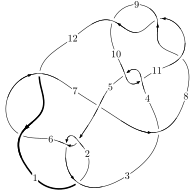
\includegraphics[width=112pt]{../../../GIT/diagram.site/Diagrams/png/1100_12a_0299.png}\\
\ \ \ A knot diagram\footnotemark}&
\allowdisplaybreaks
\textbf{Linearized knot diagam} \\
\cline{2-2}
 &
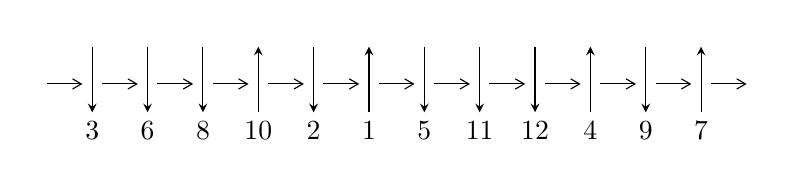
\begin{tikzpicture}[x=20pt, y=17pt]
	% nodes
	\node (C0) at (0, 0) {};
	\node (C1) at (1, 0) {};
	\node (C1U) at (1, +1) {};
	\node (C1D) at (1, -1) {3};

	\node (C2) at (2, 0) {};
	\node (C2U) at (2, +1) {};
	\node (C2D) at (2, -1) {6};

	\node (C3) at (3, 0) {};
	\node (C3U) at (3, +1) {};
	\node (C3D) at (3, -1) {8};

	\node (C4) at (4, 0) {};
	\node (C4U) at (4, +1) {};
	\node (C4D) at (4, -1) {10};

	\node (C5) at (5, 0) {};
	\node (C5U) at (5, +1) {};
	\node (C5D) at (5, -1) {2};

	\node (C6) at (6, 0) {};
	\node (C6U) at (6, +1) {};
	\node (C6D) at (6, -1) {1};

	\node (C7) at (7, 0) {};
	\node (C7U) at (7, +1) {};
	\node (C7D) at (7, -1) {5};

	\node (C8) at (8, 0) {};
	\node (C8U) at (8, +1) {};
	\node (C8D) at (8, -1) {11};

	\node (C9) at (9, 0) {};
	\node (C9U) at (9, +1) {};
	\node (C9D) at (9, -1) {12};

	\node (C10) at (10, 0) {};
	\node (C10U) at (10, +1) {};
	\node (C10D) at (10, -1) {4};

	\node (C11) at (11, 0) {};
	\node (C11U) at (11, +1) {};
	\node (C11D) at (11, -1) {9};

	\node (C12) at (12, 0) {};
	\node (C12U) at (12, +1) {};
	\node (C12D) at (12, -1) {7};
	\node (C13) at (13, 0) {};

	% arrows
	\draw[->,>={angle 60}]
	(C0) edge (C1) (C1) edge (C2) (C2) edge (C3) (C3) edge (C4) (C4) edge (C5) (C5) edge (C6) (C6) edge (C7) (C7) edge (C8) (C8) edge (C9) (C9) edge (C10) (C10) edge (C11) (C11) edge (C12) (C12) edge (C13) ;	\draw[->,>=stealth]
	(C1U) edge (C1D) (C2U) edge (C2D) (C3U) edge (C3D) (C4D) edge (C4U) (C5U) edge (C5D) (C6D) edge (C6U) (C7U) edge (C7D) (C8U) edge (C8D) (C9U) edge (C9D) (C10D) edge (C10U) (C11U) edge (C11D) (C12D) edge (C12U) ;
	\end{tikzpicture} \\
\hhline{~~} \\& 
\textbf{Solving Sequence} \\ \cline{2-2} 
 &
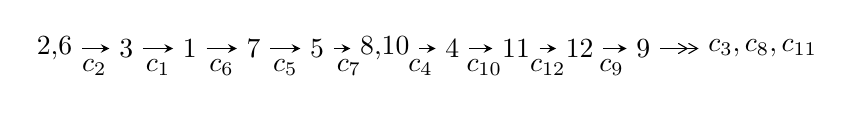
\begin{tikzpicture}[x=23pt, y=7pt]
	% node
	\node (A0) at (-1/8, 0) {2,6};
	\node (A1) at (1, 0) {3};
	\node (A2) at (2, 0) {1};
	\node (A3) at (3, 0) {7};
	\node (A4) at (4, 0) {5};
	\node (A5) at (81/16, 0) {8,10};
	\node (A6) at (49/8, 0) {4};
	\node (A7) at (57/8, 0) {11};
	\node (A8) at (65/8, 0) {12};
	\node (A9) at (73/8, 0) {9};
	\node (C1) at (1/2, -1) {$c_{2}$};
	\node (C2) at (3/2, -1) {$c_{1}$};
	\node (C3) at (5/2, -1) {$c_{6}$};
	\node (C4) at (7/2, -1) {$c_{5}$};
	\node (C5) at (9/2, -1) {$c_{7}$};
	\node (C6) at (45/8, -1) {$c_{4}$};
	\node (C7) at (53/8, -1) {$c_{10}$};
	\node (C8) at (61/8, -1) {$c_{12}$};
	\node (C9) at (69/8, -1) {$c_{9}$};
	\node (A10) at (11, 0) {$c_{3},c_{8},c_{11}$};

	% edge
	\draw[->,>=stealth]	
	(A0) edge (A1) (A1) edge (A2) (A2) edge (A3) (A3) edge (A4) (A4) edge (A5) (A5) edge (A6) (A6) edge (A7) (A7) edge (A8) (A8) edge (A9) ;
	\draw[->>,>={angle 60}]	
	(A9) edge (A10);
\end{tikzpicture} \\ 

\end{tabular} \\

\footnotetext{
The image of knot diagram is generated by the software ``\textbf{Draw programme}" developed by Andrew Bartholomew(\url{http://www.layer8.co.uk/maths/draw/index.htm\#Running-draw}), where we modified some parts for our purpose(\url{https://github.com/CATsTAILs/LinksPainter}).
}\phantom \\ \newline 
\centering \textbf{Ideals for irreducible components\footnotemark of $X_{\text{par}}$} 
 
\begin{align*}
I^u_{1}&=\langle 
u^{88}+u^{87}+\cdots+b+2 u,\;2 u^{87}- u^{86}+\cdots+a+2 u,\;u^{89}-2 u^{88}+\cdots-3 u+1\rangle \\
I^u_{2}&=\langle 
u^8+u^7-2 u^6-2 u^5+u^4+u^3+u^2+b+u,\;u^8+u^7-2 u^6-2 u^5+u^4+u^3+u^2+a+u,\\
\phantom{I^u_{2}}&\phantom{= \langle  }u^9+u^8-2 u^7-3 u^6+u^5+3 u^4+2 u^3- u-1\rangle \\
\\
\end{align*}
\raggedright * 2 irreducible components of $\dim_{\mathbb{C}}=0$, with total 98 representations.\\
\footnotetext{All coefficients of polynomials are rational numbers. But the coefficients are sometimes approximated in decimal forms when there is not enough margin.}
\newpage
\renewcommand{\arraystretch}{1}
\centering \section*{I. $I^u_{1}= \langle u^{88}+u^{87}+\cdots+b+2 u,\;2 u^{87}- u^{86}+\cdots+a+2 u,\;u^{89}-2 u^{88}+\cdots-3 u+1 \rangle$}
\flushleft \textbf{(i) Arc colorings}\\
\begin{tabular}{m{7pt} m{180pt} m{7pt} m{180pt} }
\flushright $a_{2}=$&$\begin{pmatrix}1\\0\end{pmatrix}$ \\
\flushright $a_{6}=$&$\begin{pmatrix}0\\u\end{pmatrix}$ \\
\flushright $a_{3}=$&$\begin{pmatrix}1\\u^2\end{pmatrix}$ \\
\flushright $a_{1}=$&$\begin{pmatrix}- u^2+1\\- u^4\end{pmatrix}$ \\
\flushright $a_{7}=$&$\begin{pmatrix}u^5-2 u^3+u\\u^7- u^5+u\end{pmatrix}$ \\
\flushright $a_{5}=$&$\begin{pmatrix}u\\u\end{pmatrix}$ \\
\flushright $a_{8}=$&$\begin{pmatrix}- u^9+2 u^7- u^5-2 u^3+u\\- u^9+3 u^7-3 u^5+u\end{pmatrix}$ \\
\flushright $a_{10}=$&$\begin{pmatrix}-2 u^{87}+u^{86}+\cdots+4 u^2-2 u\\- u^{88}- u^{87}+\cdots+6 u^2-2 u\end{pmatrix}$ \\
\flushright $a_{4}=$&$\begin{pmatrix}- u^{20}+5 u^{18}-11 u^{16}+10 u^{14}+2 u^{12}-13 u^{10}+9 u^8-3 u^4+u^2+1\\- u^{20}+6 u^{18}-16 u^{16}+22 u^{14}-13 u^{12}-4 u^{10}+10 u^8-4 u^6- u^4+2 u^2\end{pmatrix}$ \\
\flushright $a_{11}=$&$\begin{pmatrix}u^{86}- u^{85}+\cdots-5 u+1\\u^{88}- u^{87}+\cdots+3 u^2- u\end{pmatrix}$ \\
\flushright $a_{12}=$&$\begin{pmatrix}- u^8+3 u^6-3 u^4+1\\- u^{10}+2 u^8- u^6-2 u^4+u^2\end{pmatrix}$ \\
\flushright $a_{9}=$&$\begin{pmatrix}- u^{87}+u^{86}+\cdots-3 u+1\\- u^{87}+u^{86}+\cdots+5 u^2- u\end{pmatrix}$\\&\end{tabular}
\flushleft \textbf{(ii) Obstruction class $= -1$}\\~\\
\flushleft \textbf{(iii) Cusp Shapes $= 10 u^{88}-13 u^{87}+\cdots+23 u-17$}\\~\\
\newpage\renewcommand{\arraystretch}{1}
\flushleft \textbf{(iv) u-Polynomials at the component}\newline \\
\begin{tabular}{m{50pt}|m{274pt}}
Crossings & \hspace{64pt}u-Polynomials at each crossing \\
\hline $$\begin{aligned}c_{1}\end{aligned}$$&$\begin{aligned}
&u^{89}+48 u^{88}+\cdots+5 u+1
\end{aligned}$\\
\hline $$\begin{aligned}c_{2},c_{5}\end{aligned}$$&$\begin{aligned}
&u^{89}+2 u^{88}+\cdots-3 u-1
\end{aligned}$\\
\hline $$\begin{aligned}c_{3}\end{aligned}$$&$\begin{aligned}
&u^{89}+2 u^{88}+\cdots-65179 u-27289
\end{aligned}$\\
\hline $$\begin{aligned}c_{4},c_{10}\end{aligned}$$&$\begin{aligned}
&u^{89}+u^{88}+\cdots-1024 u-512
\end{aligned}$\\
\hline $$\begin{aligned}c_{6},c_{12}\end{aligned}$$&$\begin{aligned}
&u^{89}+6 u^{88}+\cdots+11 u+1
\end{aligned}$\\
\hline $$\begin{aligned}c_{7}\end{aligned}$$&$\begin{aligned}
&u^{89}-12 u^{88}+\cdots-4727 u+841
\end{aligned}$\\
\hline $$\begin{aligned}c_{8},c_{9},c_{11}\end{aligned}$$&$\begin{aligned}
&u^{89}-10 u^{88}+\cdots+9 u-1
\end{aligned}$\\
\hline
\end{tabular}\\~\\
\newpage\renewcommand{\arraystretch}{1}
\flushleft \textbf{(v) Riley Polynomials at the component}\newline \\
\begin{tabular}{m{50pt}|m{274pt}}
Crossings & \hspace{64pt}Riley Polynomials at each crossing \\
\hline $$\begin{aligned}c_{1}\end{aligned}$$&$\begin{aligned}
&y^{89}-12 y^{88}+\cdots+13 y-1
\end{aligned}$\\
\hline $$\begin{aligned}c_{2},c_{5}\end{aligned}$$&$\begin{aligned}
&y^{89}-48 y^{88}+\cdots+5 y-1
\end{aligned}$\\
\hline $$\begin{aligned}c_{3}\end{aligned}$$&$\begin{aligned}
&y^{89}-48 y^{88}+\cdots+8750550417 y-744689521
\end{aligned}$\\
\hline $$\begin{aligned}c_{4},c_{10}\end{aligned}$$&$\begin{aligned}
&y^{89}+57 y^{88}+\cdots-262144 y-262144
\end{aligned}$\\
\hline $$\begin{aligned}c_{6},c_{12}\end{aligned}$$&$\begin{aligned}
&y^{89}+72 y^{88}+\cdots+173 y-1
\end{aligned}$\\
\hline $$\begin{aligned}c_{7}\end{aligned}$$&$\begin{aligned}
&y^{89}-12 y^{88}+\cdots+56852441 y-707281
\end{aligned}$\\
\hline $$\begin{aligned}c_{8},c_{9},c_{11}\end{aligned}$$&$\begin{aligned}
&y^{89}-88 y^{88}+\cdots+17 y-1
\end{aligned}$\\
\hline
\end{tabular}\\~\\
\newpage\flushleft \textbf{(vi) Complex Volumes and Cusp Shapes}
$$\begin{array}{c|c|c}  
\text{Solutions to }I^u_{1}& \I (\text{vol} + \sqrt{-1}CS) & \text{Cusp shape}\\
 \hline 
\begin{aligned}
u &= \phantom{-}0.882130 + 0.459832 I \\
a &= \phantom{-}0.753928 + 0.019303 I \\
b &= \phantom{-}1.18116 + 0.90759 I\end{aligned}
 & -1.67152 - 2.05041 I & \phantom{-0.000000 } 0 \\ \hline\begin{aligned}
u &= \phantom{-}0.882130 - 0.459832 I \\
a &= \phantom{-}0.753928 - 0.019303 I \\
b &= \phantom{-}1.18116 - 0.90759 I\end{aligned}
 & -1.67152 + 2.05041 I & \phantom{-0.000000 } 0 \\ \hline\begin{aligned}
u &= -0.888667 + 0.501711 I \\
a &= -1.68269 + 2.08780 I \\
b &= -0.63536 + 2.43657 I\end{aligned}
 & -3.19630 + 4.44922 I & \phantom{-0.000000 } 0 \\ \hline\begin{aligned}
u &= -0.888667 - 0.501711 I \\
a &= -1.68269 - 2.08780 I \\
b &= -0.63536 - 2.43657 I\end{aligned}
 & -3.19630 - 4.44922 I & \phantom{-0.000000 } 0 \\ \hline\begin{aligned}
u &= \phantom{-}0.878638 + 0.524715 I \\
a &= -2.02016 - 0.27913 I \\
b &= -2.24474 - 1.41150 I\end{aligned}
 & -0.67711 - 6.71445 I & \phantom{-0.000000 } 0 \\ \hline\begin{aligned}
u &= \phantom{-}0.878638 - 0.524715 I \\
a &= -2.02016 + 0.27913 I \\
b &= -2.24474 + 1.41150 I\end{aligned}
 & -0.67711 + 6.71445 I & \phantom{-0.000000 } 0 \\ \hline\begin{aligned}
u &= -1.025820 + 0.036404 I \\
a &= \phantom{-}0.502695 - 0.628539 I \\
b &= \phantom{-}0.32711 - 1.73815 I\end{aligned}
 & -4.46205 + 2.45218 I & \phantom{-0.000000 } 0 \\ \hline\begin{aligned}
u &= -1.025820 - 0.036404 I \\
a &= \phantom{-}0.502695 + 0.628539 I \\
b &= \phantom{-}0.32711 + 1.73815 I\end{aligned}
 & -4.46205 - 2.45218 I & \phantom{-0.000000 } 0 \\ \hline\begin{aligned}
u &= \phantom{-}1.03027\phantom{ +0.000000I} \\
a &= \phantom{-}1.17910\phantom{ +0.000000I} \\
b &= \phantom{-}0.0366382\phantom{ +0.000000I}\end{aligned}
 & -6.56879\phantom{ +0.000000I} & \phantom{-0.000000 } 0 \\ \hline\begin{aligned}
u &= -0.813408 + 0.506521 I \\
a &= \phantom{-}0.72584 - 1.39872 I \\
b &= \phantom{-}0.04222 - 1.45621 I\end{aligned}
 & \phantom{-}1.77552 + 2.79390 I & \phantom{-0.000000 } 0\\
 \hline 
 \end{array}$$\newpage$$\begin{array}{c|c|c}  
\text{Solutions to }I^u_{1}& \I (\text{vol} + \sqrt{-1}CS) & \text{Cusp shape}\\
 \hline 
\begin{aligned}
u &= -0.813408 - 0.506521 I \\
a &= \phantom{-}0.72584 + 1.39872 I \\
b &= \phantom{-}0.04222 + 1.45621 I\end{aligned}
 & \phantom{-}1.77552 - 2.79390 I & \phantom{-0.000000 } 0 \\ \hline\begin{aligned}
u &= -0.766346 + 0.574188 I \\
a &= \phantom{-}1.27704 + 1.89699 I \\
b &= \phantom{-}1.89555 + 1.02015 I\end{aligned}
 & -1.59917 + 2.27839 I & \phantom{-0.000000 } 0 \\ \hline\begin{aligned}
u &= -0.766346 - 0.574188 I \\
a &= \phantom{-}1.27704 - 1.89699 I \\
b &= \phantom{-}1.89555 - 1.02015 I\end{aligned}
 & -1.59917 - 2.27839 I & \phantom{-0.000000 } 0 \\ \hline\begin{aligned}
u &= \phantom{-}0.890309 + 0.555777 I \\
a &= \phantom{-}2.77606 - 0.04434 I \\
b &= \phantom{-}2.96738 + 1.34186 I\end{aligned}
 & -6.80614 - 10.62200 I & \phantom{-0.000000 } 0 \\ \hline\begin{aligned}
u &= \phantom{-}0.890309 - 0.555777 I \\
a &= \phantom{-}2.77606 + 0.04434 I \\
b &= \phantom{-}2.96738 - 1.34186 I\end{aligned}
 & -6.80614 + 10.62200 I & \phantom{-0.000000 } 0 \\ \hline\begin{aligned}
u &= -1.077470 + 0.067927 I \\
a &= -0.953464 - 0.030989 I \\
b &= -0.55769 + 1.30402 I\end{aligned}
 & -11.16480 + 6.01176 I & \phantom{-0.000000 } 0 \\ \hline\begin{aligned}
u &= -1.077470 - 0.067927 I \\
a &= -0.953464 + 0.030989 I \\
b &= -0.55769 - 1.30402 I\end{aligned}
 & -11.16480 - 6.01176 I & \phantom{-0.000000 } 0 \\ \hline\begin{aligned}
u &= \phantom{-}1.005540 + 0.481619 I \\
a &= -0.59169 + 1.64061 I \\
b &= -1.41901 + 0.72669 I\end{aligned}
 & -8.38626 + 0.32211 I & \phantom{-0.000000 } 0 \\ \hline\begin{aligned}
u &= \phantom{-}1.005540 - 0.481619 I \\
a &= -0.59169 - 1.64061 I \\
b &= -1.41901 - 0.72669 I\end{aligned}
 & -8.38626 - 0.32211 I & \phantom{-0.000000 } 0 \\ \hline\begin{aligned}
u &= \phantom{-}0.879956\phantom{ +0.000000I} \\
a &= -0.438903\phantom{ +0.000000I} \\
b &= \phantom{-}0.0434340\phantom{ +0.000000I}\end{aligned}
 & -1.41507\phantom{ +0.000000I} & -6.32080\phantom{ +0.000000I}\\
 \hline 
 \end{array}$$\newpage$$\begin{array}{c|c|c}  
\text{Solutions to }I^u_{1}& \I (\text{vol} + \sqrt{-1}CS) & \text{Cusp shape}\\
 \hline 
\begin{aligned}
u &= -0.719693 + 0.498115 I \\
a &= -1.64541 - 0.16716 I \\
b &= -1.37251 + 0.55867 I\end{aligned}
 & \phantom{-}2.04791 + 1.35241 I & \phantom{-}2.73599 - 3.49653 I \\ \hline\begin{aligned}
u &= -0.719693 - 0.498115 I \\
a &= -1.64541 + 0.16716 I \\
b &= -1.37251 - 0.55867 I\end{aligned}
 & \phantom{-}2.04791 - 1.35241 I & \phantom{-}2.73599 + 3.49653 I \\ \hline\begin{aligned}
u &= \phantom{-}0.604923 + 0.586080 I \\
a &= -1.17479 - 2.59369 I \\
b &= \phantom{-}0.40029 - 1.92697 I\end{aligned}
 & -6.00205 + 6.09456 I & -5.95965 - 2.74749 I \\ \hline\begin{aligned}
u &= \phantom{-}0.604923 - 0.586080 I \\
a &= -1.17479 + 2.59369 I \\
b &= \phantom{-}0.40029 + 1.92697 I\end{aligned}
 & -6.00205 - 6.09456 I & -5.95965 + 2.74749 I \\ \hline\begin{aligned}
u &= \phantom{-}0.139683 + 0.824970 I \\
a &= \phantom{-}1.78560 + 1.23758 I \\
b &= \phantom{-}0.01328 + 1.71548 I\end{aligned}
 & -10.5541 + 11.1165 I & -9.09484 - 6.04502 I \\ \hline\begin{aligned}
u &= \phantom{-}0.139683 - 0.824970 I \\
a &= \phantom{-}1.78560 - 1.23758 I \\
b &= \phantom{-}0.01328 - 1.71548 I\end{aligned}
 & -10.5541 - 11.1165 I & -9.09484 + 6.04502 I \\ \hline\begin{aligned}
u &= \phantom{-}1.125280 + 0.324670 I \\
a &= \phantom{-}0.020945 + 1.149410 I \\
b &= -0.391515 + 0.232413 I\end{aligned}
 & -7.90994 + 0.10402 I & \phantom{-0.000000 } 0 \\ \hline\begin{aligned}
u &= \phantom{-}1.125280 - 0.324670 I \\
a &= \phantom{-}0.020945 - 1.149410 I \\
b &= -0.391515 - 0.232413 I\end{aligned}
 & -7.90994 - 0.10402 I & \phantom{-0.000000 } 0 \\ \hline\begin{aligned}
u &= \phantom{-}0.070097 + 0.824515 I \\
a &= -1.33999 - 0.65701 I \\
b &= \phantom{-}0.428690 - 0.050398 I\end{aligned}
 & -12.56960 - 1.39660 I & -11.14850 + 0.59888 I \\ \hline\begin{aligned}
u &= \phantom{-}0.070097 - 0.824515 I \\
a &= -1.33999 + 0.65701 I \\
b &= \phantom{-}0.428690 + 0.050398 I\end{aligned}
 & -12.56960 + 1.39660 I & -11.14850 - 0.59888 I\\
 \hline 
 \end{array}$$\newpage$$\begin{array}{c|c|c}  
\text{Solutions to }I^u_{1}& \I (\text{vol} + \sqrt{-1}CS) & \text{Cusp shape}\\
 \hline 
\begin{aligned}
u &= \phantom{-}0.127151 + 0.808870 I \\
a &= -1.86816 - 1.03664 I \\
b &= -0.334206 - 1.268780 I\end{aligned}
 & -4.17538 + 6.91543 I & -6.85978 - 6.00800 I \\ \hline\begin{aligned}
u &= \phantom{-}0.127151 - 0.808870 I \\
a &= -1.86816 + 1.03664 I \\
b &= -0.334206 + 1.268780 I\end{aligned}
 & -4.17538 - 6.91543 I & -6.85978 + 6.00800 I \\ \hline\begin{aligned}
u &= -0.114199 + 0.807947 I \\
a &= -0.871998 - 0.500386 I \\
b &= -0.900709 + 1.046200 I\end{aligned}
 & -6.70509 - 4.38760 I & -8.59798 + 3.04801 I \\ \hline\begin{aligned}
u &= -0.114199 - 0.807947 I \\
a &= -0.871998 + 0.500386 I \\
b &= -0.900709 - 1.046200 I\end{aligned}
 & -6.70509 + 4.38760 I & -8.59798 - 3.04801 I \\ \hline\begin{aligned}
u &= \phantom{-}0.723406 + 0.376492 I \\
a &= -0.861306 - 0.408790 I \\
b &= -0.262843 + 0.271220 I\end{aligned}
 & -1.03887 - 1.52700 I & -7.90188 + 3.36186 I \\ \hline\begin{aligned}
u &= \phantom{-}0.723406 - 0.376492 I \\
a &= -0.861306 + 0.408790 I \\
b &= -0.262843 - 0.271220 I\end{aligned}
 & -1.03887 + 1.52700 I & -7.90188 - 3.36186 I \\ \hline\begin{aligned}
u &= \phantom{-}0.100576 + 0.799788 I \\
a &= \phantom{-}1.75921 + 0.69555 I \\
b &= \phantom{-}0.308103 + 0.514595 I\end{aligned}
 & -4.99438 + 1.66944 I & -8.98744 - 0.29481 I \\ \hline\begin{aligned}
u &= \phantom{-}0.100576 - 0.799788 I \\
a &= \phantom{-}1.75921 - 0.69555 I \\
b &= \phantom{-}0.308103 - 0.514595 I\end{aligned}
 & -4.99438 - 1.66944 I & -8.98744 + 0.29481 I \\ \hline\begin{aligned}
u &= \phantom{-}0.607539 + 0.524018 I \\
a &= \phantom{-}1.23393 + 1.85731 I \\
b &= \phantom{-}0.029011 + 1.174260 I\end{aligned}
 & \phantom{-}0.07725 + 2.43549 I & -2.65496 - 3.04260 I \\ \hline\begin{aligned}
u &= \phantom{-}0.607539 - 0.524018 I \\
a &= \phantom{-}1.23393 - 1.85731 I \\
b &= \phantom{-}0.029011 - 1.174260 I\end{aligned}
 & \phantom{-}0.07725 - 2.43549 I & -2.65496 + 3.04260 I\\
 \hline 
 \end{array}$$\newpage$$\begin{array}{c|c|c}  
\text{Solutions to }I^u_{1}& \I (\text{vol} + \sqrt{-1}CS) & \text{Cusp shape}\\
 \hline 
\begin{aligned}
u &= \phantom{-}1.135680 + 0.431611 I \\
a &= -0.670399 - 0.816876 I \\
b &= -0.073487 - 0.404468 I\end{aligned}
 & -2.93289 - 1.90377 I & \phantom{-0.000000 } 0 \\ \hline\begin{aligned}
u &= \phantom{-}1.135680 - 0.431611 I \\
a &= -0.670399 + 0.816876 I \\
b &= -0.073487 + 0.404468 I\end{aligned}
 & -2.93289 + 1.90377 I & \phantom{-0.000000 } 0 \\ \hline\begin{aligned}
u &= -0.130036 + 0.763493 I \\
a &= \phantom{-}0.493983 + 0.363346 I \\
b &= \phantom{-}0.579994 - 0.453479 I\end{aligned}
 & -0.97886 - 3.00729 I & -0.67481 + 3.35384 I \\ \hline\begin{aligned}
u &= -0.130036 - 0.763493 I \\
a &= \phantom{-}0.493983 - 0.363346 I \\
b &= \phantom{-}0.579994 + 0.453479 I\end{aligned}
 & -0.97886 + 3.00729 I & -0.67481 - 3.35384 I \\ \hline\begin{aligned}
u &= -0.215646 + 0.736694 I \\
a &= \phantom{-}0.352487 - 1.192880 I \\
b &= -1.03050 - 0.98350 I\end{aligned}
 & -3.94866 - 3.37994 I & -8.08194 + 3.34507 I \\ \hline\begin{aligned}
u &= -0.215646 - 0.736694 I \\
a &= \phantom{-}0.352487 + 1.192880 I \\
b &= -1.03050 + 0.98350 I\end{aligned}
 & -3.94866 + 3.37994 I & -8.08194 - 3.34507 I \\ \hline\begin{aligned}
u &= -1.164480 + 0.443069 I \\
a &= -1.67272 + 1.68727 I \\
b &= -1.35179 + 2.31894 I\end{aligned}
 & -5.89254 + 3.02421 I & \phantom{-0.000000 } 0 \\ \hline\begin{aligned}
u &= -1.164480 - 0.443069 I \\
a &= -1.67272 - 1.68727 I \\
b &= -1.35179 - 2.31894 I\end{aligned}
 & -5.89254 - 3.02421 I & \phantom{-0.000000 } 0 \\ \hline\begin{aligned}
u &= -1.152870 + 0.481167 I \\
a &= \phantom{-}1.67874 - 0.72539 I \\
b &= \phantom{-}1.44055 - 1.35851 I\end{aligned}
 & -2.53850 + 6.10163 I & \phantom{-0.000000 } 0 \\ \hline\begin{aligned}
u &= -1.152870 - 0.481167 I \\
a &= \phantom{-}1.67874 + 0.72539 I \\
b &= \phantom{-}1.44055 + 1.35851 I\end{aligned}
 & -2.53850 - 6.10163 I & \phantom{-0.000000 } 0\\
 \hline 
 \end{array}$$\newpage$$\begin{array}{c|c|c}  
\text{Solutions to }I^u_{1}& \I (\text{vol} + \sqrt{-1}CS) & \text{Cusp shape}\\
 \hline 
\begin{aligned}
u &= \phantom{-}1.187870 + 0.391862 I \\
a &= \phantom{-}0.525322 - 0.087694 I \\
b &= \phantom{-}0.100629 + 0.162477 I\end{aligned}
 & -4.81156 - 0.89382 I & \phantom{-0.000000 } 0 \\ \hline\begin{aligned}
u &= \phantom{-}1.187870 - 0.391862 I \\
a &= \phantom{-}0.525322 + 0.087694 I \\
b &= \phantom{-}0.100629 - 0.162477 I\end{aligned}
 & -4.81156 + 0.89382 I & \phantom{-0.000000 } 0 \\ \hline\begin{aligned}
u &= \phantom{-}1.168200 + 0.464328 I \\
a &= \phantom{-}1.191870 + 0.076057 I \\
b &= \phantom{-}0.573207 - 0.271189 I\end{aligned}
 & -5.73526 - 5.29132 I & \phantom{-0.000000 } 0 \\ \hline\begin{aligned}
u &= \phantom{-}1.168200 - 0.464328 I \\
a &= \phantom{-}1.191870 - 0.076057 I \\
b &= \phantom{-}0.573207 + 0.271189 I\end{aligned}
 & -5.73526 + 5.29132 I & \phantom{-0.000000 } 0 \\ \hline\begin{aligned}
u &= -1.152500 + 0.516337 I \\
a &= -1.97753 - 0.61750 I \\
b &= -2.17920 + 0.19476 I\end{aligned}
 & -6.67800 + 8.09306 I & \phantom{-0.000000 } 0 \\ \hline\begin{aligned}
u &= -1.152500 - 0.516337 I \\
a &= -1.97753 + 0.61750 I \\
b &= -2.17920 - 0.19476 I\end{aligned}
 & -6.67800 - 8.09306 I & \phantom{-0.000000 } 0 \\ \hline\begin{aligned}
u &= -0.562722 + 0.472511 I \\
a &= \phantom{-}2.45276 - 0.28330 I \\
b &= \phantom{-}1.55804 - 1.30677 I\end{aligned}
 & -2.32225 - 0.35809 I & -4.17047 - 0.36662 I \\ \hline\begin{aligned}
u &= -0.562722 - 0.472511 I \\
a &= \phantom{-}2.45276 + 0.28330 I \\
b &= \phantom{-}1.55804 + 1.30677 I\end{aligned}
 & -2.32225 + 0.35809 I & -4.17047 + 0.36662 I \\ \hline\begin{aligned}
u &= \phantom{-}0.412453 + 0.601624 I \\
a &= -0.48507 + 1.52625 I \\
b &= -1.61234 - 0.03779 I\end{aligned}
 & -6.69419 - 4.61561 I & -6.55496 + 3.28166 I \\ \hline\begin{aligned}
u &= \phantom{-}0.412453 - 0.601624 I \\
a &= -0.48507 - 1.52625 I \\
b &= -1.61234 + 0.03779 I\end{aligned}
 & -6.69419 + 4.61561 I & -6.55496 - 3.28166 I\\
 \hline 
 \end{array}$$\newpage$$\begin{array}{c|c|c}  
\text{Solutions to }I^u_{1}& \I (\text{vol} + \sqrt{-1}CS) & \text{Cusp shape}\\
 \hline 
\begin{aligned}
u &= -1.215530 + 0.385915 I \\
a &= -1.247140 - 0.594809 I \\
b &= -0.68781 - 1.42794 I\end{aligned}
 & -8.20441 - 2.85842 I & \phantom{-0.000000 } 0 \\ \hline\begin{aligned}
u &= -1.215530 - 0.385915 I \\
a &= -1.247140 + 0.594809 I \\
b &= -0.68781 + 1.42794 I\end{aligned}
 & -8.20441 + 2.85842 I & \phantom{-0.000000 } 0 \\ \hline\begin{aligned}
u &= -1.213090 + 0.402391 I \\
a &= \phantom{-}0.473702 + 1.098800 I \\
b &= \phantom{-}0.19789 + 2.00303 I\end{aligned}
 & -8.89812 + 2.46893 I & \phantom{-0.000000 } 0 \\ \hline\begin{aligned}
u &= -1.213090 - 0.402391 I \\
a &= \phantom{-}0.473702 - 1.098800 I \\
b &= \phantom{-}0.19789 - 2.00303 I\end{aligned}
 & -8.89812 - 2.46893 I & \phantom{-0.000000 } 0 \\ \hline\begin{aligned}
u &= \phantom{-}1.216380 + 0.393944 I \\
a &= -1.033210 - 0.020800 I \\
b &= -0.130043 - 0.454382 I\end{aligned}
 & -10.68610 + 0.27825 I & \phantom{-0.000000 } 0 \\ \hline\begin{aligned}
u &= \phantom{-}1.216380 - 0.393944 I \\
a &= -1.033210 + 0.020800 I \\
b &= -0.130043 + 0.454382 I\end{aligned}
 & -10.68610 - 0.27825 I & \phantom{-0.000000 } 0 \\ \hline\begin{aligned}
u &= -1.224970 + 0.375819 I \\
a &= \phantom{-}1.393900 - 0.060385 I \\
b &= \phantom{-}0.596587 + 0.850691 I\end{aligned}
 & -14.7005 - 7.0565 I & \phantom{-0.000000 } 0 \\ \hline\begin{aligned}
u &= -1.224970 - 0.375819 I \\
a &= \phantom{-}1.393900 + 0.060385 I \\
b &= \phantom{-}0.596587 - 0.850691 I\end{aligned}
 & -14.7005 + 7.0565 I & \phantom{-0.000000 } 0 \\ \hline\begin{aligned}
u &= -1.181940 + 0.500743 I \\
a &= -0.141013 + 1.164390 I \\
b &= \phantom{-}0.368653 + 1.242040 I\end{aligned}
 & -4.04107 + 7.69031 I & \phantom{-0.000000 } 0 \\ \hline\begin{aligned}
u &= -1.181940 - 0.500743 I \\
a &= -0.141013 - 1.164390 I \\
b &= \phantom{-}0.368653 - 1.242040 I\end{aligned}
 & -4.04107 - 7.69031 I & \phantom{-0.000000 } 0\\
 \hline 
 \end{array}$$\newpage$$\begin{array}{c|c|c}  
\text{Solutions to }I^u_{1}& \I (\text{vol} + \sqrt{-1}CS) & \text{Cusp shape}\\
 \hline 
\begin{aligned}
u &= -1.226870 + 0.418077 I \\
a &= \phantom{-}0.400302 - 0.686102 I \\
b &= \phantom{-}0.48325 - 1.89392 I\end{aligned}
 & -16.4614 + 5.7289 I & \phantom{-0.000000 } 0 \\ \hline\begin{aligned}
u &= -1.226870 - 0.418077 I \\
a &= \phantom{-}0.400302 + 0.686102 I \\
b &= \phantom{-}0.48325 + 1.89392 I\end{aligned}
 & -16.4614 - 5.7289 I & \phantom{-0.000000 } 0 \\ \hline\begin{aligned}
u &= \phantom{-}1.199340 + 0.497123 I \\
a &= -1.04238 - 1.40168 I \\
b &= -1.37797 - 2.26390 I\end{aligned}
 & -8.22467 - 6.41149 I & \phantom{-0.000000 } 0 \\ \hline\begin{aligned}
u &= \phantom{-}1.199340 - 0.497123 I \\
a &= -1.04238 + 1.40168 I \\
b &= -1.37797 + 2.26390 I\end{aligned}
 & -8.22467 + 6.41149 I & \phantom{-0.000000 } 0 \\ \hline\begin{aligned}
u &= -1.200190 + 0.503588 I \\
a &= \phantom{-}0.43227 - 2.01242 I \\
b &= -0.52934 - 2.23286 I\end{aligned}
 & -9.90785 + 9.18672 I & \phantom{-0.000000 } 0 \\ \hline\begin{aligned}
u &= -1.200190 - 0.503588 I \\
a &= \phantom{-}0.43227 + 2.01242 I \\
b &= -0.52934 + 2.23286 I\end{aligned}
 & -9.90785 - 9.18672 I & \phantom{-0.000000 } 0 \\ \hline\begin{aligned}
u &= \phantom{-}1.198080 + 0.508599 I \\
a &= \phantom{-}1.91009 + 1.81162 I \\
b &= \phantom{-}1.99721 + 2.79861 I\end{aligned}
 & -7.33563 - 11.74480 I & \phantom{-0.000000 } 0 \\ \hline\begin{aligned}
u &= \phantom{-}1.198080 - 0.508599 I \\
a &= \phantom{-}1.91009 - 1.81162 I \\
b &= \phantom{-}1.99721 - 2.79861 I\end{aligned}
 & -7.33563 + 11.74480 I & \phantom{-0.000000 } 0 \\ \hline\begin{aligned}
u &= \phantom{-}1.201410 + 0.516744 I \\
a &= -2.54195 - 1.66813 I \\
b &= -2.50275 - 2.84833 I\end{aligned}
 & -13.7024 - 16.0279 I & \phantom{-0.000000 } 0 \\ \hline\begin{aligned}
u &= \phantom{-}1.201410 - 0.516744 I \\
a &= -2.54195 + 1.66813 I \\
b &= -2.50275 + 2.84833 I\end{aligned}
 & -13.7024 + 16.0279 I & \phantom{-0.000000 } 0\\
 \hline 
 \end{array}$$\newpage$$\begin{array}{c|c|c}  
\text{Solutions to }I^u_{1}& \I (\text{vol} + \sqrt{-1}CS) & \text{Cusp shape}\\
 \hline 
\begin{aligned}
u &= \phantom{-}1.214120 + 0.487768 I \\
a &= \phantom{-}0.960915 + 0.219353 I \\
b &= \phantom{-}1.64886 + 1.19641 I\end{aligned}
 & -15.9643 - 3.3550 I & \phantom{-0.000000 } 0 \\ \hline\begin{aligned}
u &= \phantom{-}1.214120 - 0.487768 I \\
a &= \phantom{-}0.960915 - 0.219353 I \\
b &= \phantom{-}1.64886 - 1.19641 I\end{aligned}
 & -15.9643 + 3.3550 I & \phantom{-0.000000 } 0 \\ \hline\begin{aligned}
u &= \phantom{-}0.045537 + 0.676922 I \\
a &= \phantom{-}1.077040 - 0.256080 I \\
b &= \phantom{-}0.256695 - 1.092910 I\end{aligned}
 & -2.59868 + 1.01996 I & -7.42495 + 0.64864 I \\ \hline\begin{aligned}
u &= \phantom{-}0.045537 - 0.676922 I \\
a &= \phantom{-}1.077040 + 0.256080 I \\
b &= \phantom{-}0.256695 + 1.092910 I\end{aligned}
 & -2.59868 - 1.01996 I & -7.42495 - 0.64864 I \\ \hline\begin{aligned}
u &= -0.143647 + 0.650890 I \\
a &= -0.915631 + 0.433122 I \\
b &= \phantom{-}0.091936 + 0.985043 I\end{aligned}
 & \phantom{-}0.32466 - 1.74343 I & -0.09678 + 4.11913 I \\ \hline\begin{aligned}
u &= -0.143647 - 0.650890 I \\
a &= -0.915631 - 0.433122 I \\
b &= \phantom{-}0.091936 - 0.985043 I\end{aligned}
 & \phantom{-}0.32466 + 1.74343 I & -0.09678 - 4.11913 I \\ \hline\begin{aligned}
u &= \phantom{-}0.379396 + 0.460960 I \\
a &= -0.230295 - 1.120240 I \\
b &= \phantom{-}0.664172 + 0.181918 I\end{aligned}
 & -0.53005 - 1.55644 I & -3.23373 + 4.26726 I \\ \hline\begin{aligned}
u &= \phantom{-}0.379396 - 0.460960 I \\
a &= -0.230295 + 1.120240 I \\
b &= \phantom{-}0.664172 - 0.181918 I\end{aligned}
 & -0.53005 + 1.55644 I & -3.23373 - 4.26726 I \\ \hline\begin{aligned}
u &= -0.557461\phantom{ +0.000000I} \\
a &= \phantom{-}2.83655\phantom{ +0.000000I} \\
b &= \phantom{-}1.80666\phantom{ +0.000000I}\end{aligned}
 & -2.28508\phantom{ +0.000000I} & -1.20430\phantom{ +0.000000I}\\
 \hline 
 \end{array}$$\newpage\newpage\renewcommand{\arraystretch}{1}
\centering \section*{II. $I^u_{2}= \langle u^8+u^7-2 u^6-2 u^5+u^4+u^3+u^2+b+u,\;u^8+u^7-2 u^6-2 u^5+u^4+u^3+u^2+a+u,\;u^9+u^8-2 u^7-3 u^6+u^5+3 u^4+2 u^3- u-1 \rangle$}
\flushleft \textbf{(i) Arc colorings}\\
\begin{tabular}{m{7pt} m{180pt} m{7pt} m{180pt} }
\flushright $a_{2}=$&$\begin{pmatrix}1\\0\end{pmatrix}$ \\
\flushright $a_{6}=$&$\begin{pmatrix}0\\u\end{pmatrix}$ \\
\flushright $a_{3}=$&$\begin{pmatrix}1\\u^2\end{pmatrix}$ \\
\flushright $a_{1}=$&$\begin{pmatrix}- u^2+1\\- u^4\end{pmatrix}$ \\
\flushright $a_{7}=$&$\begin{pmatrix}u^5-2 u^3+u\\u^7- u^5+u\end{pmatrix}$ \\
\flushright $a_{5}=$&$\begin{pmatrix}u\\u\end{pmatrix}$ \\
\flushright $a_{8}=$&$\begin{pmatrix}u^8-3 u^6+3 u^4-1\\u^8+u^7-3 u^6-2 u^5+3 u^4+2 u^3-1\end{pmatrix}$ \\
\flushright $a_{10}=$&$\begin{pmatrix}- u^8- u^7+2 u^6+2 u^5- u^4- u^3- u^2- u\\- u^8- u^7+2 u^6+2 u^5- u^4- u^3- u^2- u\end{pmatrix}$ \\
\flushright $a_{4}=$&$\begin{pmatrix}u\\u\end{pmatrix}$ \\
\flushright $a_{11}=$&$\begin{pmatrix}- u^8- u^7+2 u^6+2 u^5- u^4- u^3- u^2- u\\- u^8- u^7+2 u^6+2 u^5- u^4- u^3- u^2- u\end{pmatrix}$ \\
\flushright $a_{12}=$&$\begin{pmatrix}- u^8+3 u^6-3 u^4+1\\- u^8- u^7+3 u^6+2 u^5-3 u^4-2 u^3+1\end{pmatrix}$ \\
\flushright $a_{9}=$&$\begin{pmatrix}- u^7- u^6+2 u^5+2 u^4- u^3- u^2- u-1\\- u^6+2 u^4+u^3- u^2- u-1\end{pmatrix}$\\&\end{tabular}
\flushleft \textbf{(ii) Obstruction class $= 1$}\\~\\
\flushleft \textbf{(iii) Cusp Shapes $= - u^8-6 u^7+u^6+12 u^5+5 u^4-10 u^3-7 u^2-7 u-6$}\\~\\
\newpage\renewcommand{\arraystretch}{1}
\flushleft \textbf{(iv) u-Polynomials at the component}\newline \\
\begin{tabular}{m{50pt}|m{274pt}}
Crossings & \hspace{64pt}u-Polynomials at each crossing \\
\hline $$\begin{aligned}c_{1}\end{aligned}$$&$\begin{aligned}
&u^9-5 u^8+12 u^7-15 u^6+9 u^5+u^4-4 u^3+2 u^2+u-1
\end{aligned}$\\
\hline $$\begin{aligned}c_{2}\end{aligned}$$&$\begin{aligned}
&u^9+u^8-2 u^7-3 u^6+u^5+3 u^4+2 u^3- u-1
\end{aligned}$\\
\hline $$\begin{aligned}c_{3}\end{aligned}$$&$\begin{aligned}
&u^9+u^8+2 u^7+u^6+3 u^5+u^4+2 u^3+u-1
\end{aligned}$\\
\hline $$\begin{aligned}c_{4},c_{10}\end{aligned}$$&$\begin{aligned}
&u^9
\end{aligned}$\\
\hline $$\begin{aligned}c_{5}\end{aligned}$$&$\begin{aligned}
&u^9- u^8-2 u^7+3 u^6+u^5-3 u^4+2 u^3- u+1
\end{aligned}$\\
\hline $$\begin{aligned}c_{6}\end{aligned}$$&$\begin{aligned}
&u^9-3 u^8+8 u^7-13 u^6+17 u^5-17 u^4+12 u^3-6 u^2+u+1
\end{aligned}$\\
\hline $$\begin{aligned}c_{7}\end{aligned}$$&$\begin{aligned}
&u^9- u^8+2 u^7- u^6+3 u^5- u^4+2 u^3+u+1
\end{aligned}$\\
\hline $$\begin{aligned}c_{8},c_{9}\end{aligned}$$&$\begin{aligned}
&(u-1)^9
\end{aligned}$\\
\hline $$\begin{aligned}c_{11}\end{aligned}$$&$\begin{aligned}
&(u+1)^9
\end{aligned}$\\
\hline $$\begin{aligned}c_{12}\end{aligned}$$&$\begin{aligned}
&u^9+3 u^8+8 u^7+13 u^6+17 u^5+17 u^4+12 u^3+6 u^2+u-1
\end{aligned}$\\
\hline
\end{tabular}\\~\\
\newpage\renewcommand{\arraystretch}{1}
\flushleft \textbf{(v) Riley Polynomials at the component}\newline \\
\begin{tabular}{m{50pt}|m{274pt}}
Crossings & \hspace{64pt}Riley Polynomials at each crossing \\
\hline $$\begin{aligned}c_{1}\end{aligned}$$&$\begin{aligned}
&y^9- y^8+12 y^7-7 y^6+37 y^5+y^4-10 y^2+5 y-1
\end{aligned}$\\
\hline $$\begin{aligned}c_{2},c_{5}\end{aligned}$$&$\begin{aligned}
&y^9-5 y^8+12 y^7-15 y^6+9 y^5+y^4-4 y^3+2 y^2+y-1
\end{aligned}$\\
\hline $$\begin{aligned}c_{3},c_{7}\end{aligned}$$&$\begin{aligned}
&y^9+3 y^8+8 y^7+13 y^6+17 y^5+17 y^4+12 y^3+6 y^2+y-1
\end{aligned}$\\
\hline $$\begin{aligned}c_{4},c_{10}\end{aligned}$$&$\begin{aligned}
&y^9
\end{aligned}$\\
\hline $$\begin{aligned}c_{6},c_{12}\end{aligned}$$&$\begin{aligned}
&y^9+7 y^8+20 y^7+25 y^6+5 y^5-15 y^4+22 y^2+13 y-1
\end{aligned}$\\
\hline $$\begin{aligned}c_{8},c_{9},c_{11}\end{aligned}$$&$\begin{aligned}
&(y-1)^9
\end{aligned}$\\
\hline
\end{tabular}\\~\\
\newpage\flushleft \textbf{(vi) Complex Volumes and Cusp Shapes}
$$\begin{array}{c|c|c}  
\text{Solutions to }I^u_{2}& \I (\text{vol} + \sqrt{-1}CS) & \text{Cusp shape}\\
 \hline 
\begin{aligned}
u &= -0.772920 + 0.510351 I \\
a &= \phantom{-}0.630598 + 0.707882 I \\
b &= \phantom{-}0.630598 + 0.707882 I\end{aligned}
 & \phantom{-}0.13850 + 2.09337 I & -1.56547 - 4.18932 I \\ \hline\begin{aligned}
u &= -0.772920 - 0.510351 I \\
a &= \phantom{-}0.630598 - 0.707882 I \\
b &= \phantom{-}0.630598 - 0.707882 I\end{aligned}
 & \phantom{-}0.13850 - 2.09337 I & -1.56547 + 4.18932 I \\ \hline\begin{aligned}
u &= \phantom{-}0.825933\phantom{ +0.000000I} \\
a &= -1.61202\phantom{ +0.000000I} \\
b &= -1.61202\phantom{ +0.000000I}\end{aligned}
 & -2.84338\phantom{ +0.000000I} & -16.7240\phantom{ +0.000000I} \\ \hline\begin{aligned}
u &= \phantom{-}1.173910 + 0.391555 I \\
a &= \phantom{-}0.552775 + 1.001020 I \\
b &= \phantom{-}0.552775 + 1.001020 I\end{aligned}
 & -6.01628 - 1.33617 I & -11.45029 + 1.01794 I \\ \hline\begin{aligned}
u &= \phantom{-}1.173910 - 0.391555 I \\
a &= \phantom{-}0.552775 - 1.001020 I \\
b &= \phantom{-}0.552775 - 1.001020 I\end{aligned}
 & -6.01628 + 1.33617 I & -11.45029 - 1.01794 I \\ \hline\begin{aligned}
u &= -0.141484 + 0.739668 I \\
a &= -0.481040 - 0.507127 I \\
b &= -0.481040 - 0.507127 I\end{aligned}
 & -2.26187 - 2.45442 I & -5.68179 + 2.62939 I \\ \hline\begin{aligned}
u &= -0.141484 - 0.739668 I \\
a &= -0.481040 + 0.507127 I \\
b &= -0.481040 + 0.507127 I\end{aligned}
 & -2.26187 + 2.45442 I & -5.68179 - 2.62939 I \\ \hline\begin{aligned}
u &= -1.172470 + 0.500383 I \\
a &= -0.896321 - 0.526299 I \\
b &= -0.896321 - 0.526299 I\end{aligned}
 & -5.24306 + 7.08493 I & -8.94033 - 5.11095 I \\ \hline\begin{aligned}
u &= -1.172470 - 0.500383 I \\
a &= -0.896321 + 0.526299 I \\
b &= -0.896321 + 0.526299 I\end{aligned}
 & -5.24306 - 7.08493 I & -8.94033 + 5.11095 I\\
 \hline 
 \end{array}$$\newpage
\newpage\renewcommand{\arraystretch}{1}
\centering \section*{ III. u-Polynomials}
\begin{tabular}{m{50pt}|m{274pt}}
Crossings & \hspace{64pt}u-Polynomials at each crossing \\
\hline $$\begin{aligned}c_{1}\end{aligned}$$&$\begin{aligned}
&(u^9-5 u^8+12 u^7-15 u^6+9 u^5+u^4-4 u^3+2 u^2+u-1)\\
&\cdot(u^{89}+48 u^{88}+\cdots+5 u+1)
\end{aligned}$\\
\hline $$\begin{aligned}c_{2}\end{aligned}$$&$\begin{aligned}
&(u^9+u^8+\cdots- u-1)(u^{89}+2 u^{88}+\cdots-3 u-1)
\end{aligned}$\\
\hline $$\begin{aligned}c_{3}\end{aligned}$$&$\begin{aligned}
&(u^9+u^8+2 u^7+u^6+3 u^5+u^4+2 u^3+u-1)\\
&\cdot(u^{89}+2 u^{88}+\cdots-65179 u-27289)
\end{aligned}$\\
\hline $$\begin{aligned}c_{4},c_{10}\end{aligned}$$&$\begin{aligned}
&u^9(u^{89}+u^{88}+\cdots-1024 u-512)
\end{aligned}$\\
\hline $$\begin{aligned}c_{5}\end{aligned}$$&$\begin{aligned}
&(u^9- u^8+\cdots- u+1)(u^{89}+2 u^{88}+\cdots-3 u-1)
\end{aligned}$\\
\hline $$\begin{aligned}c_{6}\end{aligned}$$&$\begin{aligned}
&(u^9-3 u^8+8 u^7-13 u^6+17 u^5-17 u^4+12 u^3-6 u^2+u+1)\\
&\cdot(u^{89}+6 u^{88}+\cdots+11 u+1)
\end{aligned}$\\
\hline $$\begin{aligned}c_{7}\end{aligned}$$&$\begin{aligned}
&(u^9- u^8+2 u^7- u^6+3 u^5- u^4+2 u^3+u+1)\\
&\cdot(u^{89}-12 u^{88}+\cdots-4727 u+841)
\end{aligned}$\\
\hline $$\begin{aligned}c_{8},c_{9}\end{aligned}$$&$\begin{aligned}
&((u-1)^9)(u^{89}-10 u^{88}+\cdots+9 u-1)
\end{aligned}$\\
\hline $$\begin{aligned}c_{11}\end{aligned}$$&$\begin{aligned}
&((u+1)^9)(u^{89}-10 u^{88}+\cdots+9 u-1)
\end{aligned}$\\
\hline $$\begin{aligned}c_{12}\end{aligned}$$&$\begin{aligned}
&(u^9+3 u^8+8 u^7+13 u^6+17 u^5+17 u^4+12 u^3+6 u^2+u-1)\\
&\cdot(u^{89}+6 u^{88}+\cdots+11 u+1)
\end{aligned}$\\
\hline
\end{tabular}\newpage\renewcommand{\arraystretch}{1}
\centering \section*{ IV. Riley Polynomials}
\begin{tabular}{m{50pt}|m{274pt}}
Crossings & \hspace{64pt}Riley Polynomials at each crossing \\
\hline $$\begin{aligned}c_{1}\end{aligned}$$&$\begin{aligned}
&(y^9- y^8+12 y^7-7 y^6+37 y^5+y^4-10 y^2+5 y-1)\\
&\cdot(y^{89}-12 y^{88}+\cdots+13 y-1)
\end{aligned}$\\
\hline $$\begin{aligned}c_{2},c_{5}\end{aligned}$$&$\begin{aligned}
&(y^9-5 y^8+12 y^7-15 y^6+9 y^5+y^4-4 y^3+2 y^2+y-1)\\
&\cdot(y^{89}-48 y^{88}+\cdots+5 y-1)
\end{aligned}$\\
\hline $$\begin{aligned}c_{3}\end{aligned}$$&$\begin{aligned}
&(y^9+3 y^8+8 y^7+13 y^6+17 y^5+17 y^4+12 y^3+6 y^2+y-1)\\
&\cdot(y^{89}-48 y^{88}+\cdots+8750550417 y-744689521)
\end{aligned}$\\
\hline $$\begin{aligned}c_{4},c_{10}\end{aligned}$$&$\begin{aligned}
&y^9(y^{89}+57 y^{88}+\cdots-262144 y-262144)
\end{aligned}$\\
\hline $$\begin{aligned}c_{6},c_{12}\end{aligned}$$&$\begin{aligned}
&(y^9+7 y^8+20 y^7+25 y^6+5 y^5-15 y^4+22 y^2+13 y-1)\\
&\cdot(y^{89}+72 y^{88}+\cdots+173 y-1)
\end{aligned}$\\
\hline $$\begin{aligned}c_{7}\end{aligned}$$&$\begin{aligned}
&(y^9+3 y^8+8 y^7+13 y^6+17 y^5+17 y^4+12 y^3+6 y^2+y-1)\\
&\cdot(y^{89}-12 y^{88}+\cdots+56852441 y-707281)
\end{aligned}$\\
\hline $$\begin{aligned}c_{8},c_{9},c_{11}\end{aligned}$$&$\begin{aligned}
&((y-1)^9)(y^{89}-88 y^{88}+\cdots+17 y-1)
\end{aligned}$\\
\hline
\end{tabular}
\vskip 2pc
\end{document}